\section{Artefact removal}




\begin{figure}[!htbp]
\minipage{.5\textwidth}%
\centering
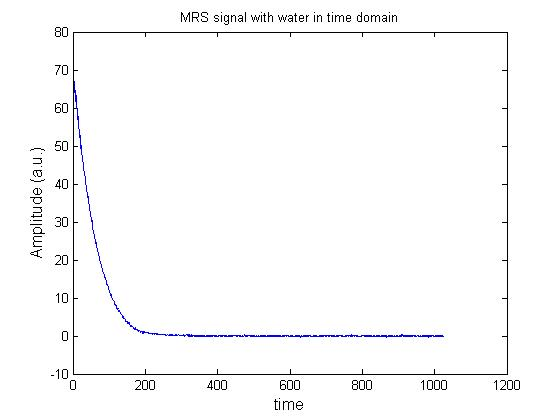
\includegraphics[width=.8\textwidth]{1.jpg}
\subcaption{Acquire signal in time domain}\label{1}
\endminipage\hfill
\minipage{.5\textwidth}%
\centering
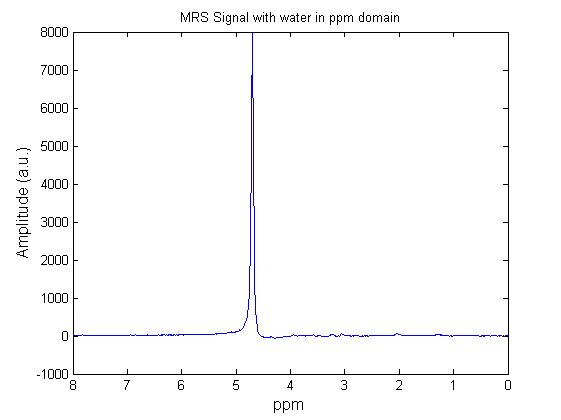
\includegraphics[width=.8\textwidth]{2.jpg}
\subcaption{Spectrum of the signal in ppm}\label{2}
\endminipage\hfill
\caption{The raw signal acquired from the MRS}
\end{figure}

 
Each component is exponentially damped complex-valued sinusoid of Lorentz type equation \ref{eq1}.


\begin{figure}[!htbp]
\minipage{.5\textwidth}%
\centering

\includegraphics[width=.8\textwidth]{3.jpg}
\subcaption{K component of the signal in time domain}\label{3}
\endminipage\hfill
\minipage{.5\textwidth}%
\centering
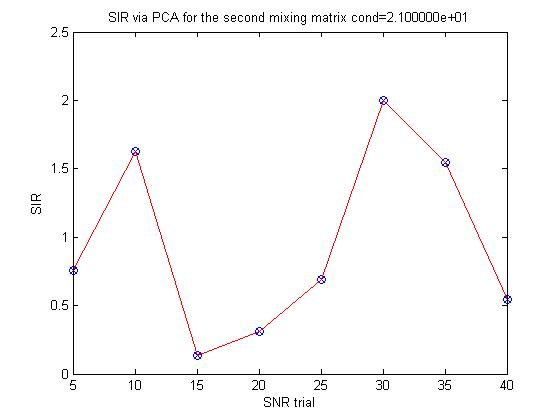
\includegraphics[width=.8\textwidth]{4.jpg}
\subcaption{Spectrum of the K component}\label{4}
\endminipage\hfill
\caption{Herein different metabolite component are extracted into individual part}
\end{figure}

The critical point is removing water is determination of components K which is related to the number of pics in the main spectrum. A reasonable number is required for a good SNR since underestimated K might omit the necessary pics to be suppressed. On the other hand a very large K could generate unwanted spectrum including noise component\cite{1}. 

\begin{equation}
SNR=20*\log\bigg\{\frac{OriginalSignal}{FilteredSignal-OriginalSignal}\bigg\}
\end{equation} 

In order estimate the number of needed components from the figure \ref{Nad1} there is a clear plot of the signal-to-noise ration versus the total number of components estimated. The SNR value theoretically should be as big as possible. This confirm that the extract signal has far more higher amplitude compare to the noise that was canceled out from the subspace filtering \cite{1}.

\begin{figure}[!htbp]
\centering
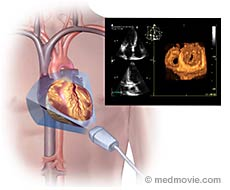
\includegraphics[width=1\textwidth]{5.jpg}
\caption{Spectrum components}\label{fig1}
\end{figure}

In the figure \ref{fig1} are the individual component where 30 is the model order. Herein it is notable that the central frequency increases as for at high order. After the suppression of the water components the spectrum of the filtered signal outcome has the pattern as in figure \ref{fig2}. Since the analysis was performed across different order the SNR estimation tends to stabilize at order higher than 19. In order to have the best cumulative estimation 30 as model order has been assigned throughout the following tasks. However it will be concluded into the third part of this session that for model lower than 30 the estimation is less accurate. Moreover the component with a central frequency sitting at higher than $4.7 ppm$ has to be suppressed. This component are displayed in both time and frequency domain respectively in figure \ref{fig5} and \ref{fig4} at \ref{S1A1}. 

The filtering has also been observed in model order. The results ate figure \ref{fig6} and \ref{fig7} indicate that high model order tends to include all possible peaks at the desired frequencies lower than $4.7ppm$. Another important fact is that watter peak is significantly high compare to the other metabolites. This is mainly due to the fact that watter composition in the body is $80\%$. Consequently by suppressing this peaks the relative scale in the plot will go down drastically and makes possible the other peaks to be very obvious fig \ref{fig2}. 


\begin{figure}[!htbp]

\minipage{.5\textwidth}%
\centering
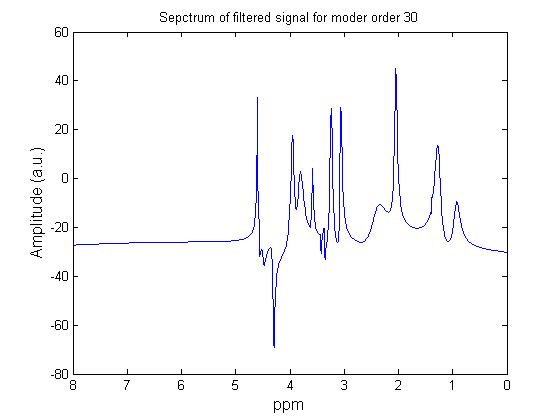
\includegraphics[width=1\textwidth]{8_1.jpg}
\subcaption{Spectrum Water filtered signal for model order 30}\label{fig2}
\endminipage\hfill
\minipage{.5\textwidth}%
\centering
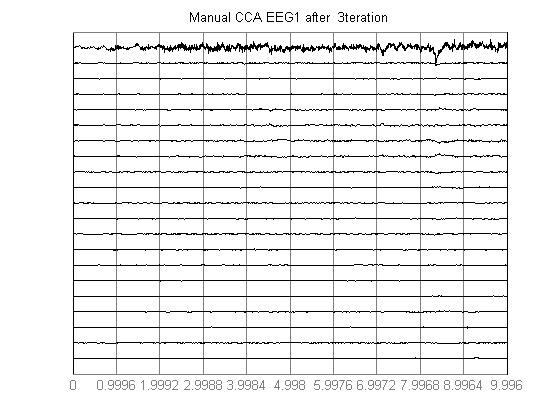
\includegraphics[width=1\textwidth]{11.jpg}
\subcaption{Signal-to-noise ration for different model order}\label{Nad1}
\endminipage\hfill
\caption{Cleaned signal from the water interference resided in the MRS spectrum fig \ref{1}}
\end{figure}

\newpage
\subsection{Comparison with classical filters}

Subspace filtering is a very powerful toolbox for noise removal composed of advantages and drawbacks compared to the other existing classical approaches such as spectral subtraction and Wiener filtering. Spectral extraction is restricted into a fixed FFT computational whereas SVD based topologies vary in computational time with the  Karhunen–Loève Transform data. In addition KLT transform $O(nm^2)$ is far more heavy in terms of computation compare to FFT $O(nlog(n))$ \cite{2}.

Moreover in this content subspace algorithm assume explicitly the order of the signal, or in other word the rank-deficient speech observation matrix. Whereas Wiener filtering does an implicit rank reduction based on a estimation of rank reduced correlation matrix \cite{2}.

Apart from the fft spectral approach, DCT is another candidate for signal enhancement yet it is far superior compare to the theoretical subspace filtering\cite{2}.

The benefits of using subspace filtering consist mainly on lower level of distortion when the signal is projected into the subspace with the minimum residue noise. Similarly the spectral extraction filter distort the desired signal but the residue level in this case is significantly higher resulting into low SNR level. Thus a moderation of signal distortion and nulling noisy component makes subspace algorithm superior to the classical filtering topologies \cite{3}.  

Another important aspect is the prior knowledge. This is an almost totally useless information for the classical filter. In the subspace case it increases the accuracy of parameter estimation and thus an higher SNR could be possible\cite{3}.

Differently from the classical filters, subspace approach efficiency depend significantly on the ability of the user to identify the accurately the characteristics of the underlying signal. The better the properties are defined the better the removal of the noises is performed\cite{5}. The other classical filters require no need of any additional visualization skills therefore are mostly applied in fully automated systems.

In order to consistently apply the subspace filtering, the signal has to be modelled into a clear analytical formulation. In some modalities this is not a very easy task consequently its application is restricted into very well known physical models.

Another fundamental issue with subspaces signal is that noise incorporated in the signal which needs to be reduced is considered white. In case of narrow band noises a pre-whitening step has to be applied before the the filtering itself takes place \cite{6}.


